% !TeX root = ../main.tex
\cleardoublepage
\chapter{其他有参考价值的内容}


%%% mashup

\begin{sidewaysfigure}[p]
  \centering
  \begin{minipage}{\textwidth}
    \centering
    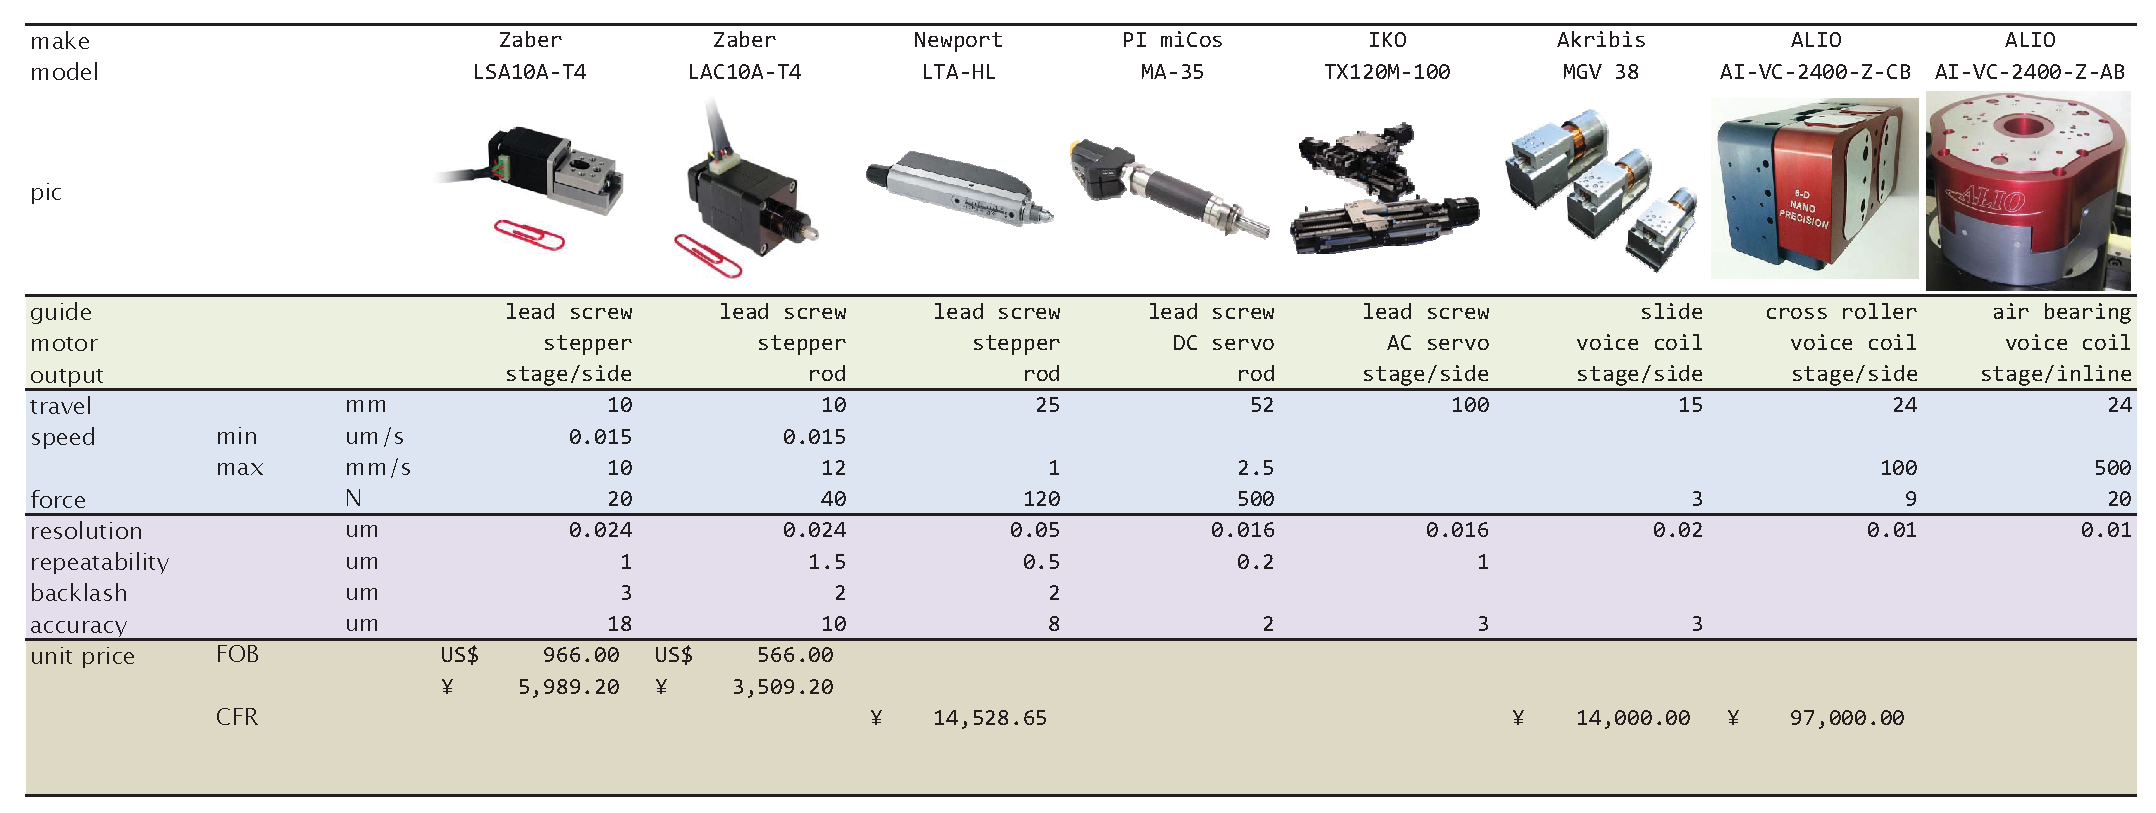
\includegraphics
      [max size={\textwidth}{0.9\textheight}]
      {_b/mashup__feeding}
    \caption{精密直线进给机构选型表(\ref{sec:rig-probe-feeding}节)}
    \label{fig:-b-mashup-feeding}
  \end{minipage}%
  \par\bigskip
  \begin{minipage}{\textwidth}
    \centering
    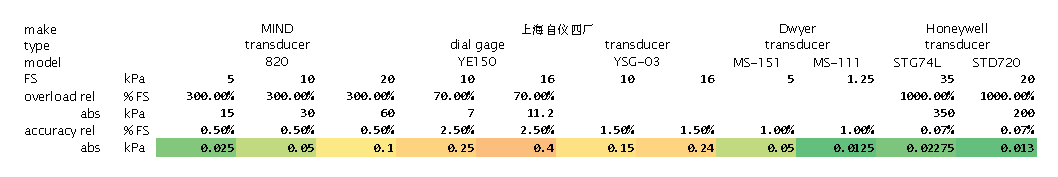
\includegraphics
      [max size={\textwidth}{0.9\textheight}]
      {_b/mashup__pressure}
    \caption{压强变送器选型表(\ref{sec:rig-pressure-sensor}节)}
    \label{fig:-b-mashup-pressure}
  \end{minipage}
\end{sidewaysfigure}


%%% pcb

\begin{sidewaysfigure}[p]
\centering
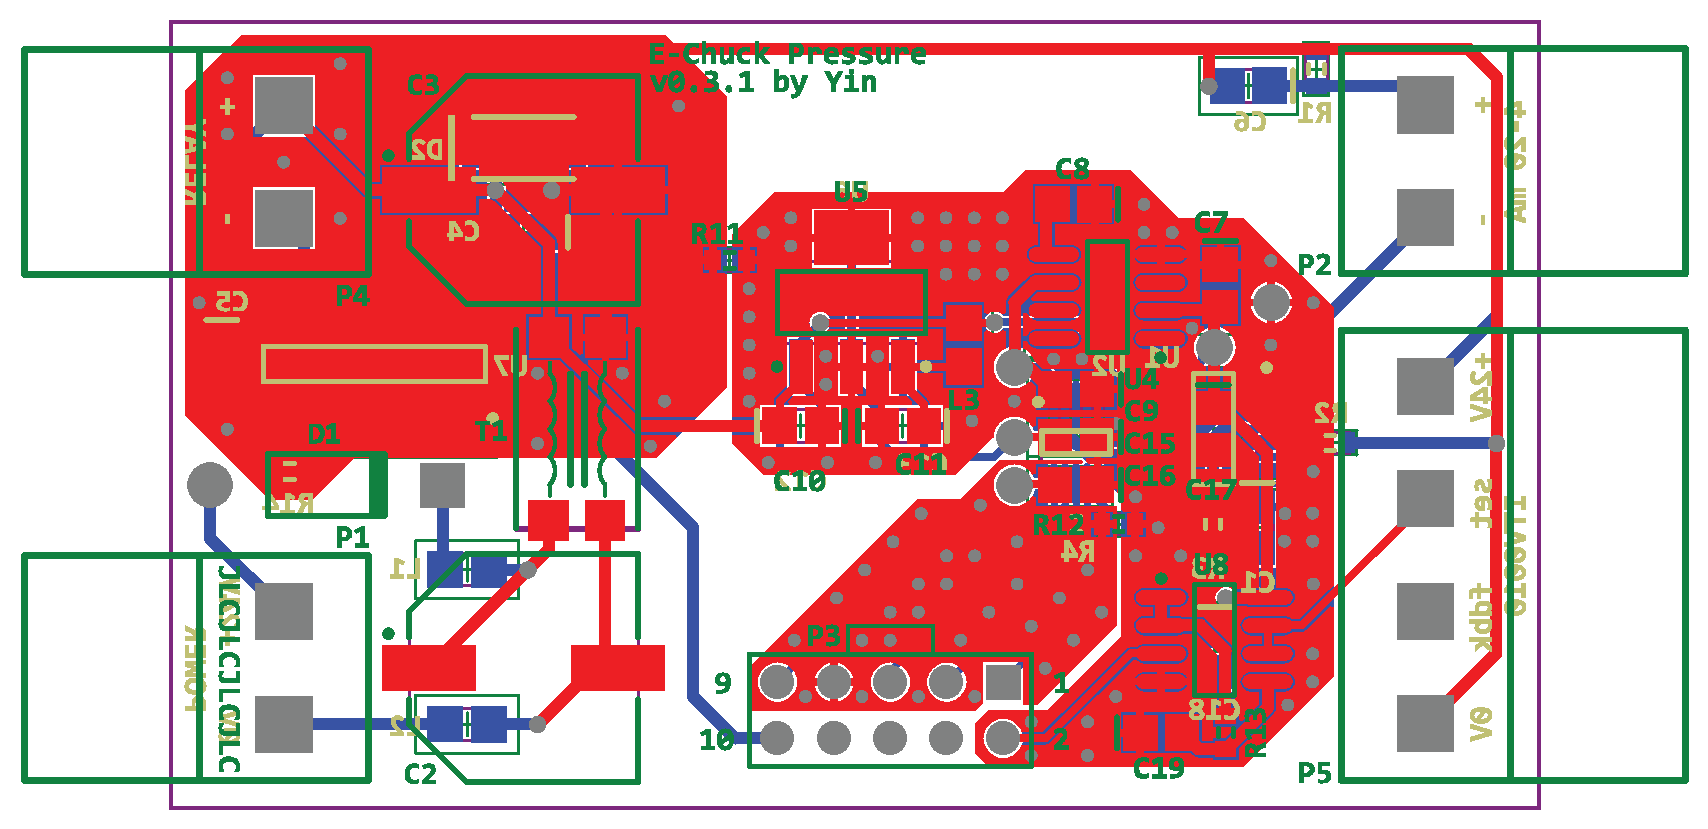
\includegraphics
  [max size={\textwidth}{0.9\textheight}]
  {_b/pcb__pressure}
\caption{背吹控制系统接口PCB布线图(\ref{sec:impl-pcb-pressure}节)}
\label{fig:-b-pcb-pressure}
\end{sidewaysfigure}

\begin{figure}[p]
\centering
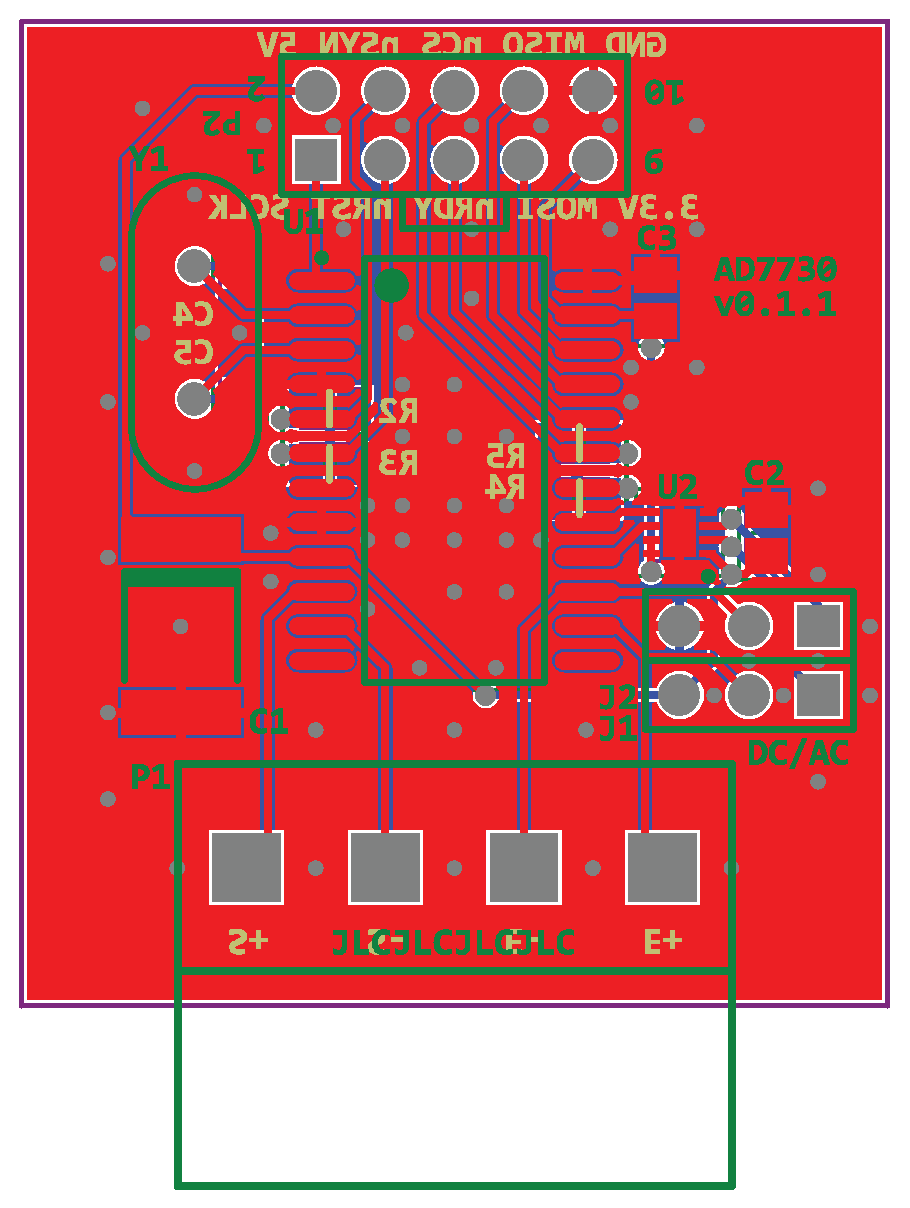
\includegraphics
  [max size={\textwidth}{0.9\textheight}]
  {_b/pcb__ad7730}
\caption{微力传感器接口PCB布线图(\ref{sec:impl-pcb-ad7730}节)}
\label{fig:-b-pcb-ad7730}
\end{figure}

\begin{figure}[p]
\centering
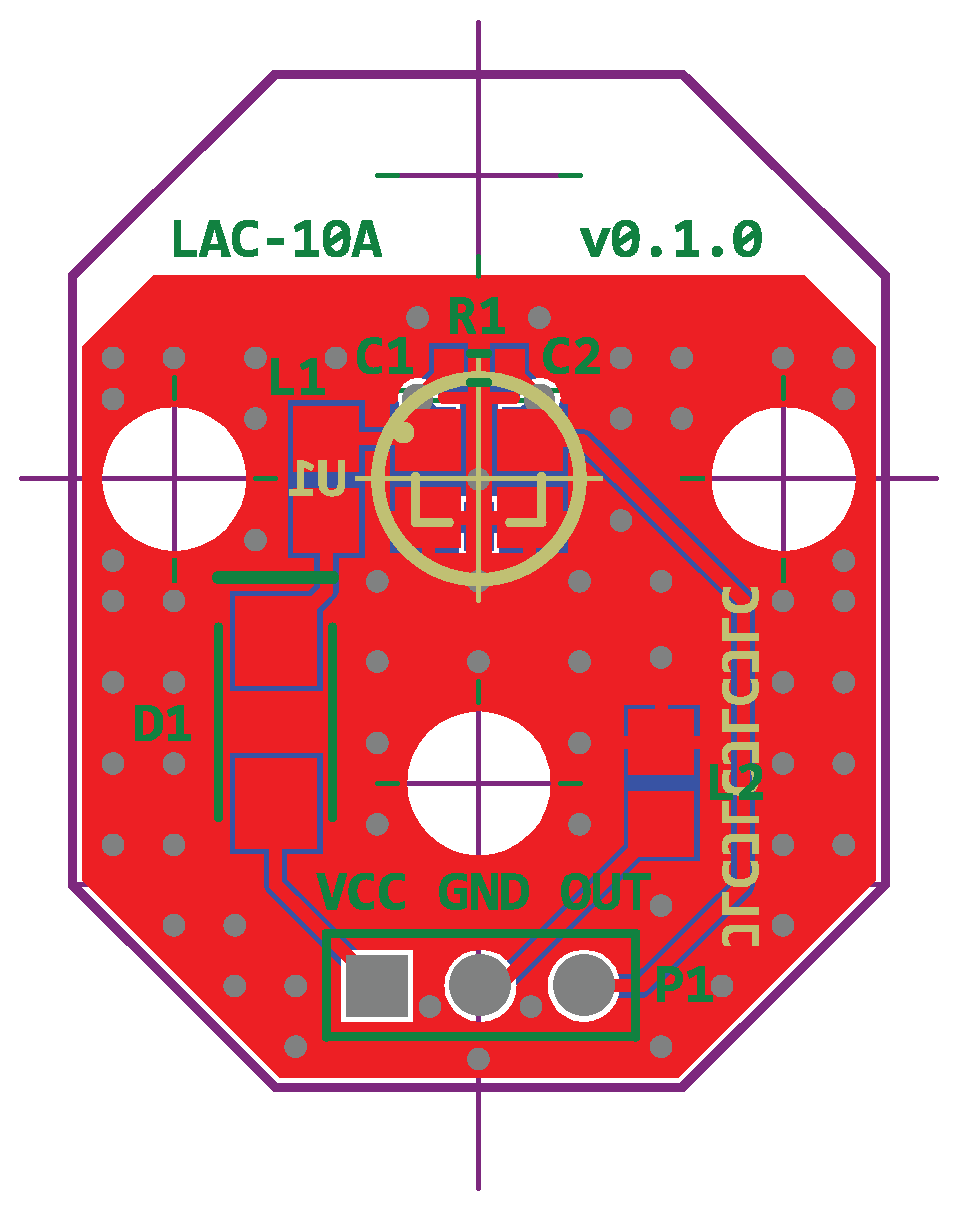
\includegraphics
  [max size={\textwidth}{0.9\textheight}]
  {_b/pcb__zaber}
\caption{LAC-10A零位传感器PCB布线图(\ref{sec:impl-pcb-zaber-homing}节)}
\label{fig:-b-pcb-zaber}
\end{figure}